%*******10********20********30********40********50********60********70********80

% For all chapters, use the newdefined chap{} instead of chapter{}
% This will make the text at the top-left of the page be the same as the chapter
\doublespacing
\chap{Introduction}
   
In recent years, there has been a lot of research going on in the area of deep learning. It has paved a path for solving many abstruse problems in the field of computer vision such as self driving cars, human facial expression detection\cite{1612.02903}, object recognition etc. Convolutional neural network have become so powerful that they have outperformed humans in some object recognition \cite{CNN-Better,krizhevsky2012imagenet,szegedy2015going,he2016deep,simonyan2014very} test. For many years deep learning was considered a black box as it has innumerable interacting, non linear parts. To study what each of its neurons has learned to detect is to visualize when does each neurons is triggered.  
Many researcher have worked and presented various techniques and results about how does CNNs are able to work so well. 

Development of many tools and techniques have enabled researchers to visualize and interpret the hidden layers of neural networks. This not only has enabled researchers to improve CNNs for various supervised learning algorithms but also use to them in different unsupervised learning tasks \cite{1506.06579}. 

\par

Image generative models have been used for a wide variety of problems such as applying various fancy filters to images, compression and decompression of images, super resolution \cite{1609.04802} and image inpainting \cite{1607.07539}.
 One of the major advantages for image generation is the easy availability and accessibility  of image repositories \cite{celeba} , so it does not require labeled dataset.

\begin{figure}[H]
  \centering
    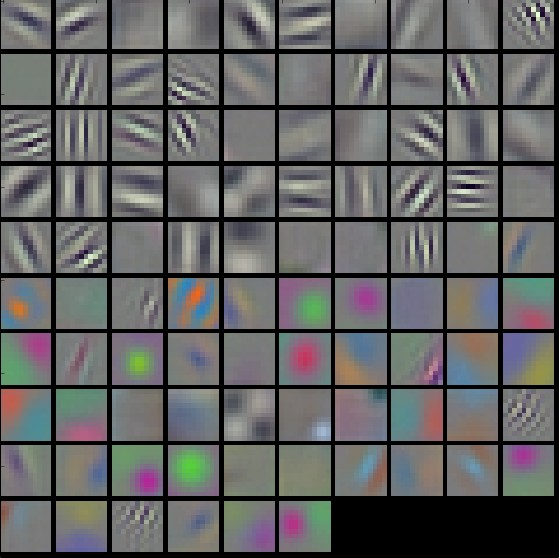
\includegraphics[scale=.3, angle=0]{Files/cnn_visaulize.jpeg}
    \caption[Typical-looking filters on the first CONV layer of a imagenet]{Typical-looking filters on the first CONV layer}
    \label{fig:visualize-cnn}
\end{figure}








\section{Synthetic Image Generation}
Image generation is one the central research area under the category of unsupervised learning. To understand unsupervised learning, lets look at supervised learning first. In supervised learning, when given data and its label we try to model a function which learns the mapping of data to its label. A complexity of data grows , it becomes very hard to model a function that can cover all the features of the data. Deep learning takes advantage of this with higher-level learned
features defined in terms of lower-level features \cite{bengio2012deep}. In other words, we are trying to find the posterior probability distribution of an object in an image, $P(y|x)$.
In unsupervised learning, we are given the data sample but we don't have the target or the output label. In unsupervised learning, the model tries understand and model the whole data. There are several unsupervised machine learning algorithms such as KNN, clustering etc. Hence, image generation problem falls under the category of unsupervised learning where the we are trying to mimic the distribution of images present in the dataset. In this work, we have synthesised the images based on some given conditions. Most widely used method before Generative Adversarial Network involved using probabilistic generative models which are discussed in section 2.1. This work uses Generative Adversarial Network framework for image generation which was first introduced by Goodfellow \textit{et al.} \cite{Original-GAN}. But the proposed  framework is highly unstable and generated low quality images. This work focuses on the aspect of stabilising and reviewing the latest GAN frameworks.

\section{Motivation}


The CNN have shown excellent capability in classification task\cite{CNN-Better} but they require large amount of labeled data. Labeling and gathering large data require lot of human effort and money. This work tries to reduce this by developing generative model which are capable of generating labeled data.
There has been lot of research going on area in the area of generative framework. After the first paper there have been lot of papers which have modified and tweaked the framework to produce quality data sample. There are various frameworks which have tried various approaches to make GAN work. 

\section{Organization}

To explain this work, we start with  \autoref{chap:RelatedWork}. In this chapter we look at various work done in field of generative model and also look at different models based on generative adversarial network. In the next \autoref{chap:CNN} we look at the key building block of this work, which is perceptron and later convolutional neural Network. Then in next \autoref{chap:GAN} we explain the concept of generative adversarial framework. Now once we understood the GAN we look at modification done as part of this work in \autoref{chap:EGAN}. Later in \autoref{chap:result}, we look at some of the experiments and result obtained when framework shown in \autoref{chap:EGAN} is implemented.